%%%%%%%%%%%%%%%%%%%%%%%%%%%%%%%%%%%%%%%%%
% NIWeek 2014 Poster by T. Reveyrand
% www.microwave.fr
% http://www.microwave.fr/LaTeX.html
% ---------------------------------------
% 
% Original template created by:
% Brian Amberg (baposter@brian-amberg.de)
%
% This template has been downloaded from:
% http://www.LaTeXTemplates.com
%
% License:
% CC BY-NC-SA 3.0 (http://creativecommons.org/licenses/by-nc-sa/3.0/)
%
%%%%%%%%%%%%%%%%%%%%%%%%%%%%%%%%%%%%%%%%%

%----------------------------------------------------------------------------------------
%	PACKAGES AND OTHER DOCUMENT CONFIGURATIONS
%----------------------------------------------------------------------------------------

\documentclass[a0paper,portrait]{baposter}

\usepackage[font=small,labelfont=bf]{caption} % Required for specifying captions to tables and figures
\usepackage{booktabs} % Horizontal rules in tables
\usepackage{relsize} % Used for making text smaller in some places
\usepackage{makecell}
\usepackage{amsmath,amsfonts,amssymb,amsthm} % Math packages
\usepackage{eqparbox}

\usepackage{textcomp}


\usepackage{bm}


\graphicspath{{figures/}} % Directory in which figures are stored

\definecolor{bordercol}{RGB}{40,40,40} % Border color of content boxes
\definecolor{headercol1}{RGB}{186,215,230} % Background color for the header in the content boxes (left side)
\definecolor{headercol2}{RGB}{120,120,120} % Background color for the header in the content boxes (right side)
\definecolor{headerfontcol}{RGB}{0,0,0} % Text color for the header text in the content boxes
\definecolor{boxcolor}{RGB}{255,255,255} % Background color for the content in the content boxes


\begin{document}

\background{ % Set the background to an image (background.pdf)
    \begin{tikzpicture}[remember picture,overlay]
        \draw (current page.north west)+(-2em,2em) node[anchor=north west]
        {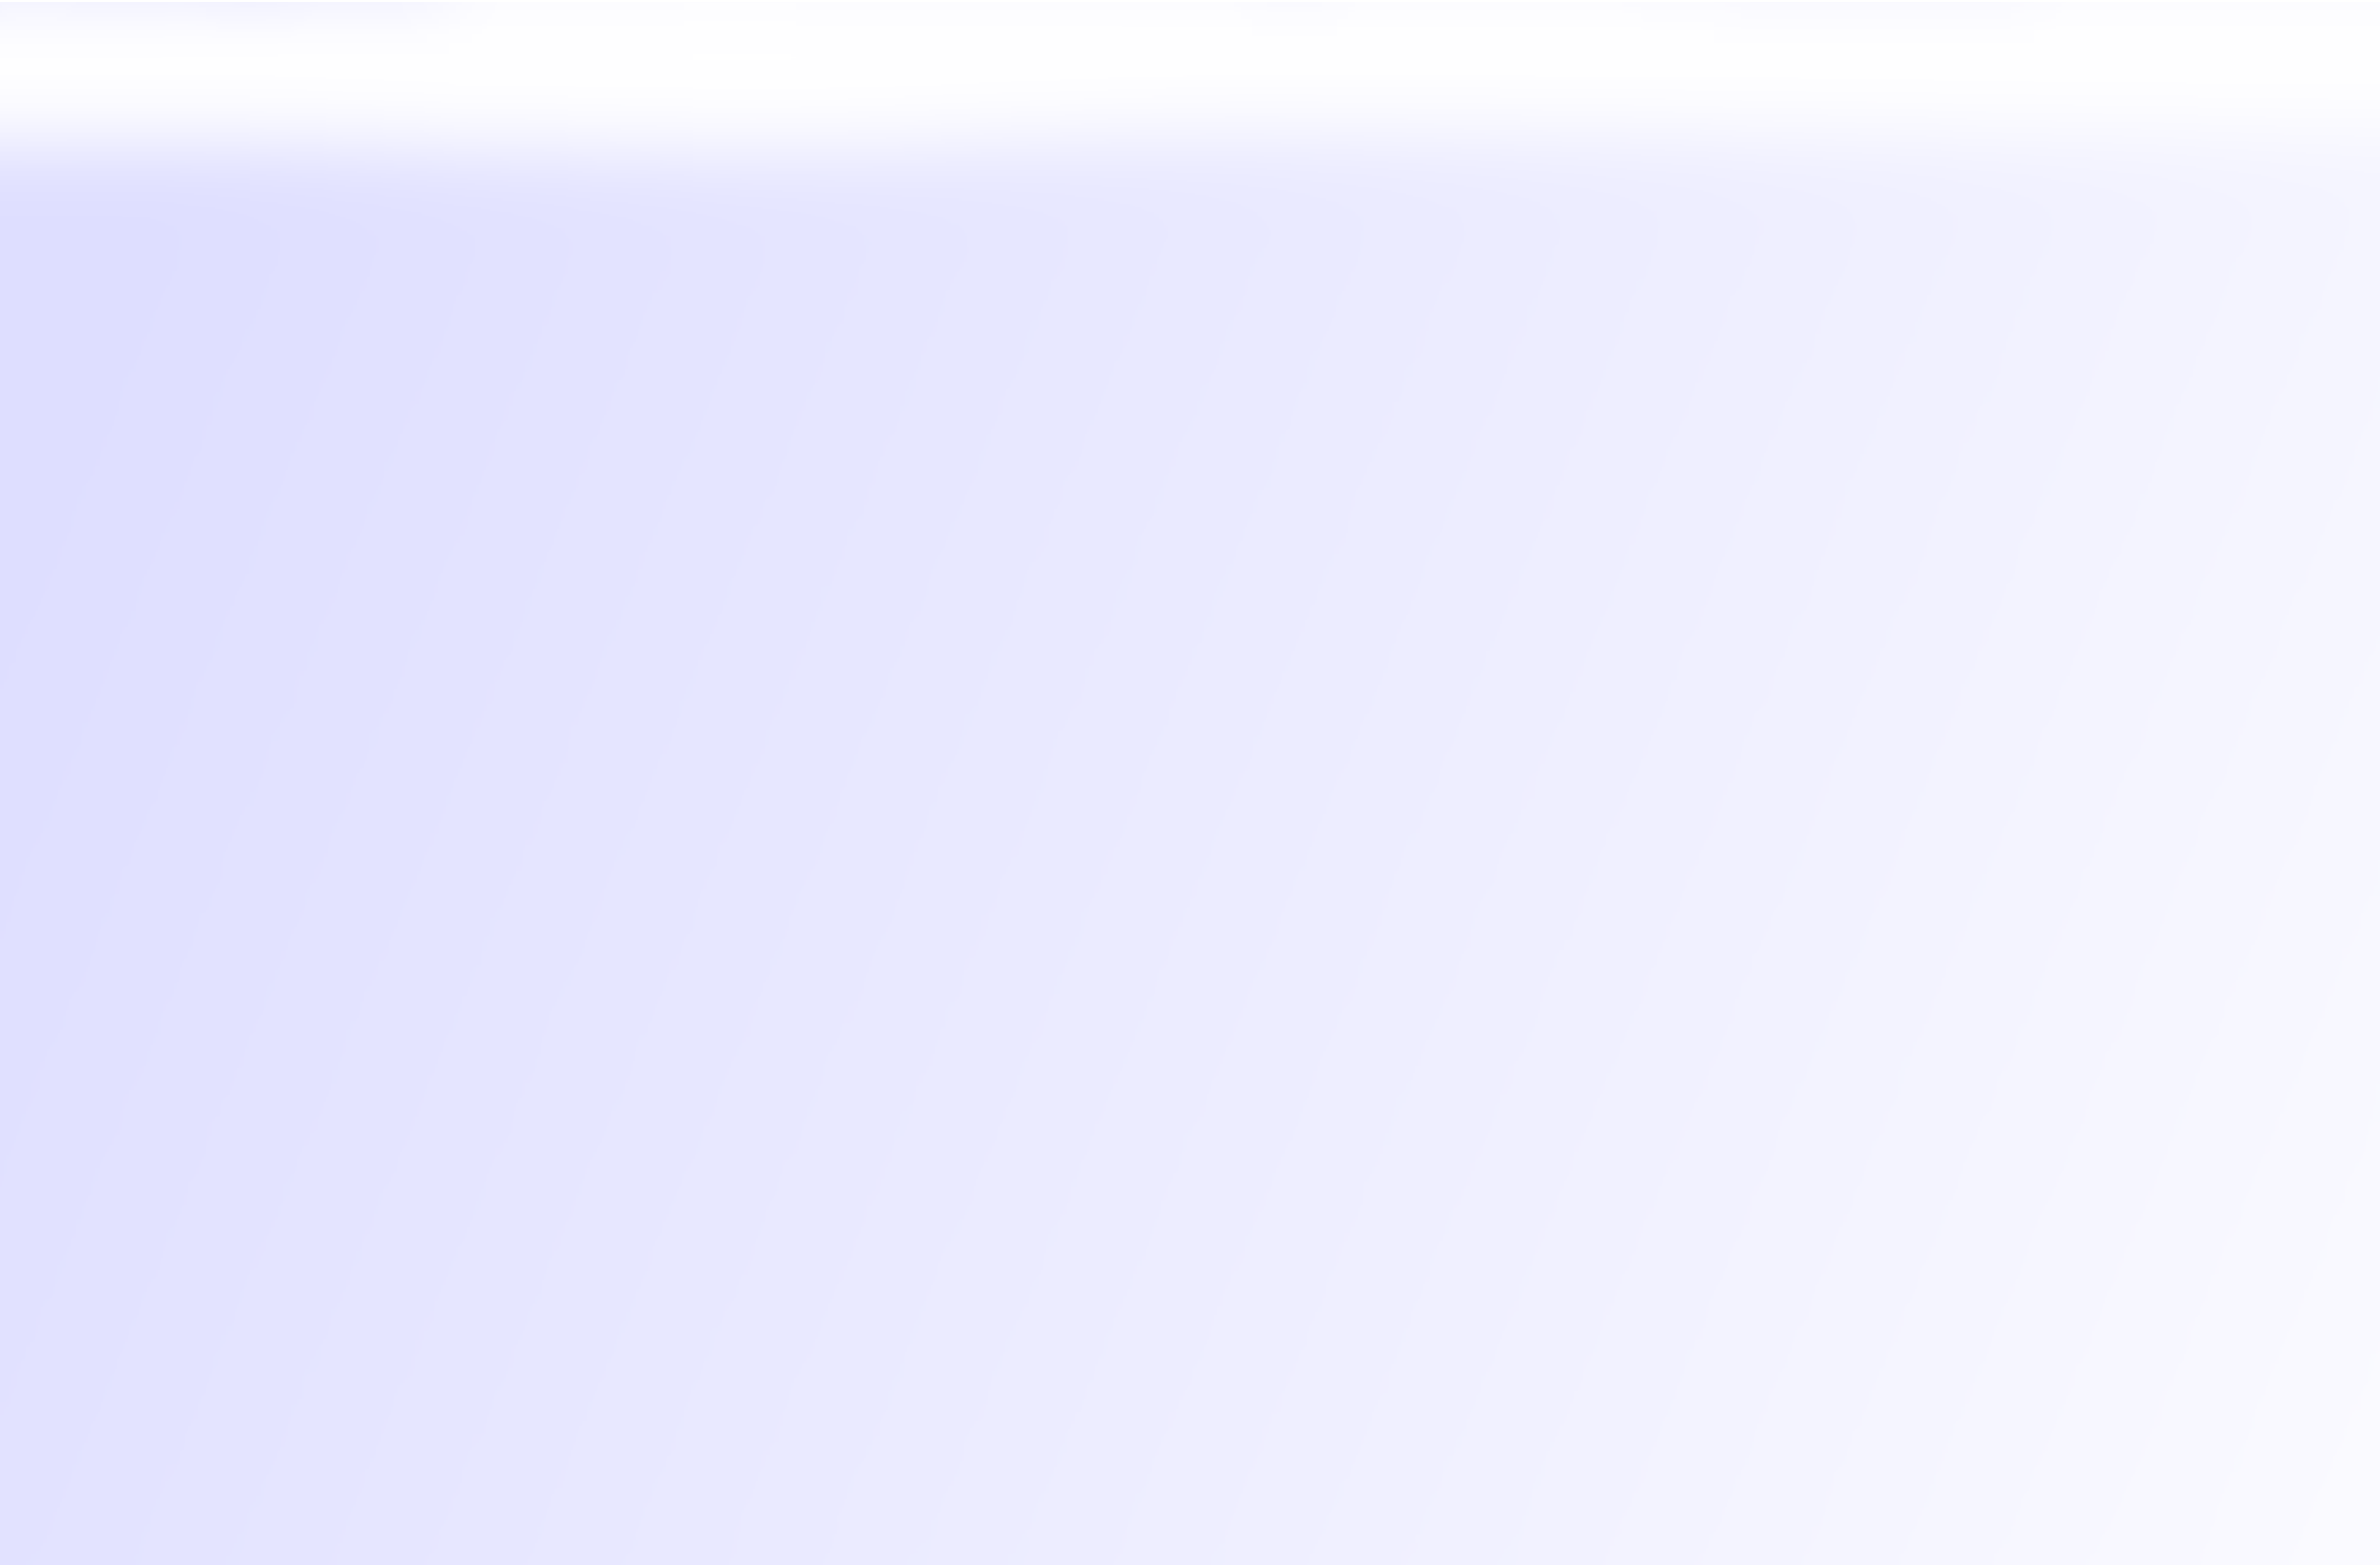
\includegraphics[height=1.1\textheight]{background}};
    \end{tikzpicture}
}

\begin{poster}{
    columns=2,
    grid=false,
    borderColor=bordercol, % Border color of content boxes
    headerColorOne=headercol1, % Background color for the header in the content boxes (left side)
    headerColorTwo=headercol2, % Background color for the header in the content boxes (right side)
    headerFontColor=headerfontcol, % Text color for the header text in the content boxes
    boxColorOne=boxcolor, % Background color for the content in the content boxes
    headershape=roundedright, % Specify the rounded corner in the content box headers
    headerfont=\Large\sf\bf, % Font modifiers for the text in the content box headers
    textborder=rectangle,
    background=user,
    headerborder=open, % Change to closed for a line under the content box headers
    boxshade=plain
}
{
\includegraphics[scale=0.17]{epfl.png}}
%
%
%----------------------------------------------------------------------------------------
%	TITLE AND AUTHOR NAME
%----------------------------------------------------------------------------------------
{ \bf  \huge {Embedding Memory into Advanced Dialogue Management}} % Poster title
{\vspace{0.3em} \smaller Chia-An Yu\\  % Author names
  
\smaller {Under the supervision of Pr. Martin Jaggi, Dr. Claudiu Musat} \\ EPFL } % Author email addresses
{
\includegraphics[scale=0.058]{swisscom.png}} % University/lab logo


%----------------------------------------------------------------------------------------
%	INTRODUCTION
%----------------------------------------------------------------------------------------
\headerbox{Introduction}{name=introduction,column=0,row=0,span=2}{
    \begin{itemize}
        \item This project focuses on frame tracking \cite{asri2017frames}, a way to incorporate memory into a goal-oriented dialogue system.
        \item We propose a model with attention mechanism that is inspired by how human resolves frame references.
        \item We introduce a method to generate synthetic frame tracking data and use the data for pre-training.
    \end{itemize}
}


%----------------------------------------------------------------------------------------
%	FRAME-TRACKING
%----------------------------------------------------------------------------------------
\headerbox{Frame tracking}{name=frame-tracking,column=0,below=introduction}{
    \begin{itemize}
        \item In a goal-oriented dialogue, a frame summarizes an option for the user. It is represented as a list of slot-value pairs.
        \item The goal of frame tracking is to find out the most related frame for each natural language tag in the utterance.
        \item We use FRAMES dataset \cite{asri2017frames} as the training set.
        \\
    \end{itemize}
    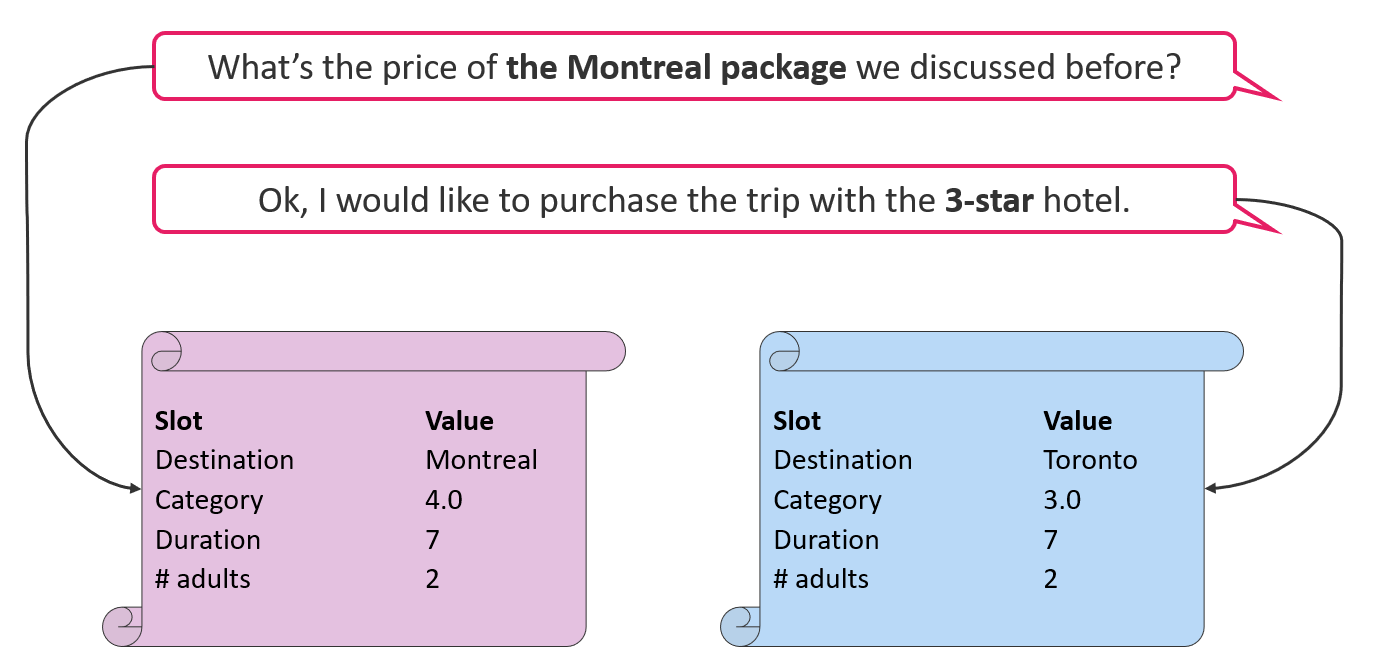
\includegraphics[width=\columnwidth]{frame-tracking.png}
}


%----------------------------------------------------------------------------------------
%	SYNTHETIC DATASET
%----------------------------------------------------------------------------------------
\headerbox{Synthetic datasets}{name=synthetic,column=0,below=frame-tracking}{
    \begin{itemize}
        \item We generate synthetic frame tracking data by interleaving dialogues from MultiWOZ, a large dataset without frame tracking labels.
        \item We transform dialogue state labels into frames, and create synthetic frame references.
    \end{itemize}
    \begin{center}
        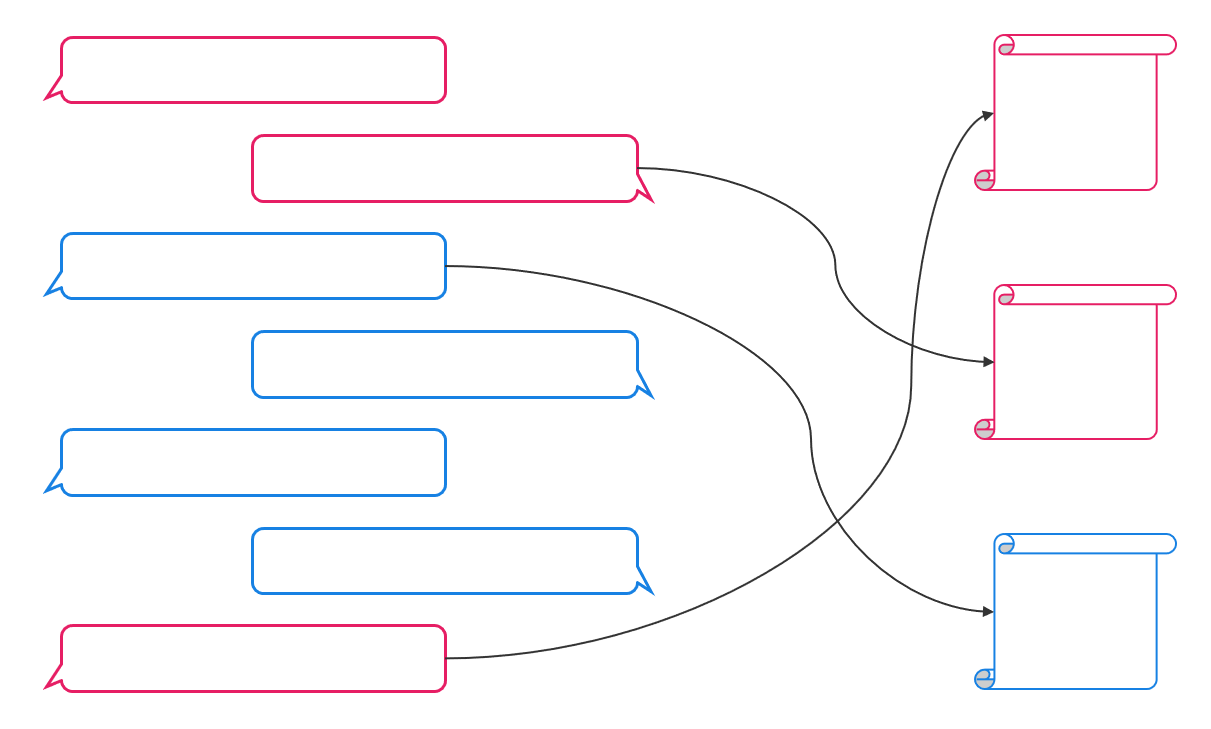
\includegraphics[width=0.7\columnwidth]{synthetic.png}
    \end{center}
    \begin{center}
        \begin{tabular}{lrl}
            \toprule
            Dataset & \# dialogues & Domain(s) \\
            \midrule
            FRAMES & 1369 & Hotel + flight \\
            Synthetic 1 & 5488 & Single domain \\
            Synthetic 2 & 3820 & Hotel + restaurant \\
            Synthetic 3 & 3820 & Hotel + transportation (taxi and train) \\
            \bottomrule
        \end{tabular}
    \end{center}
}


%----------------------------------------------------------
%	MODEL
%----------------------------------------------------------------------------------------
\headerbox{Model}{name=model,column=1,row=1,below=introduction,span=1}{
    \begin{itemize}
        \item We use a lookup table for act and slot embedding.
        \item We consider two types of text embedding for value tags: pre-trained BERT feature and GRU-based embedding training from scratch.
        \item We experiment with several attention mechanisms, including dot product, query-key attention, etc.
    \end{itemize}
    \begin{center}
        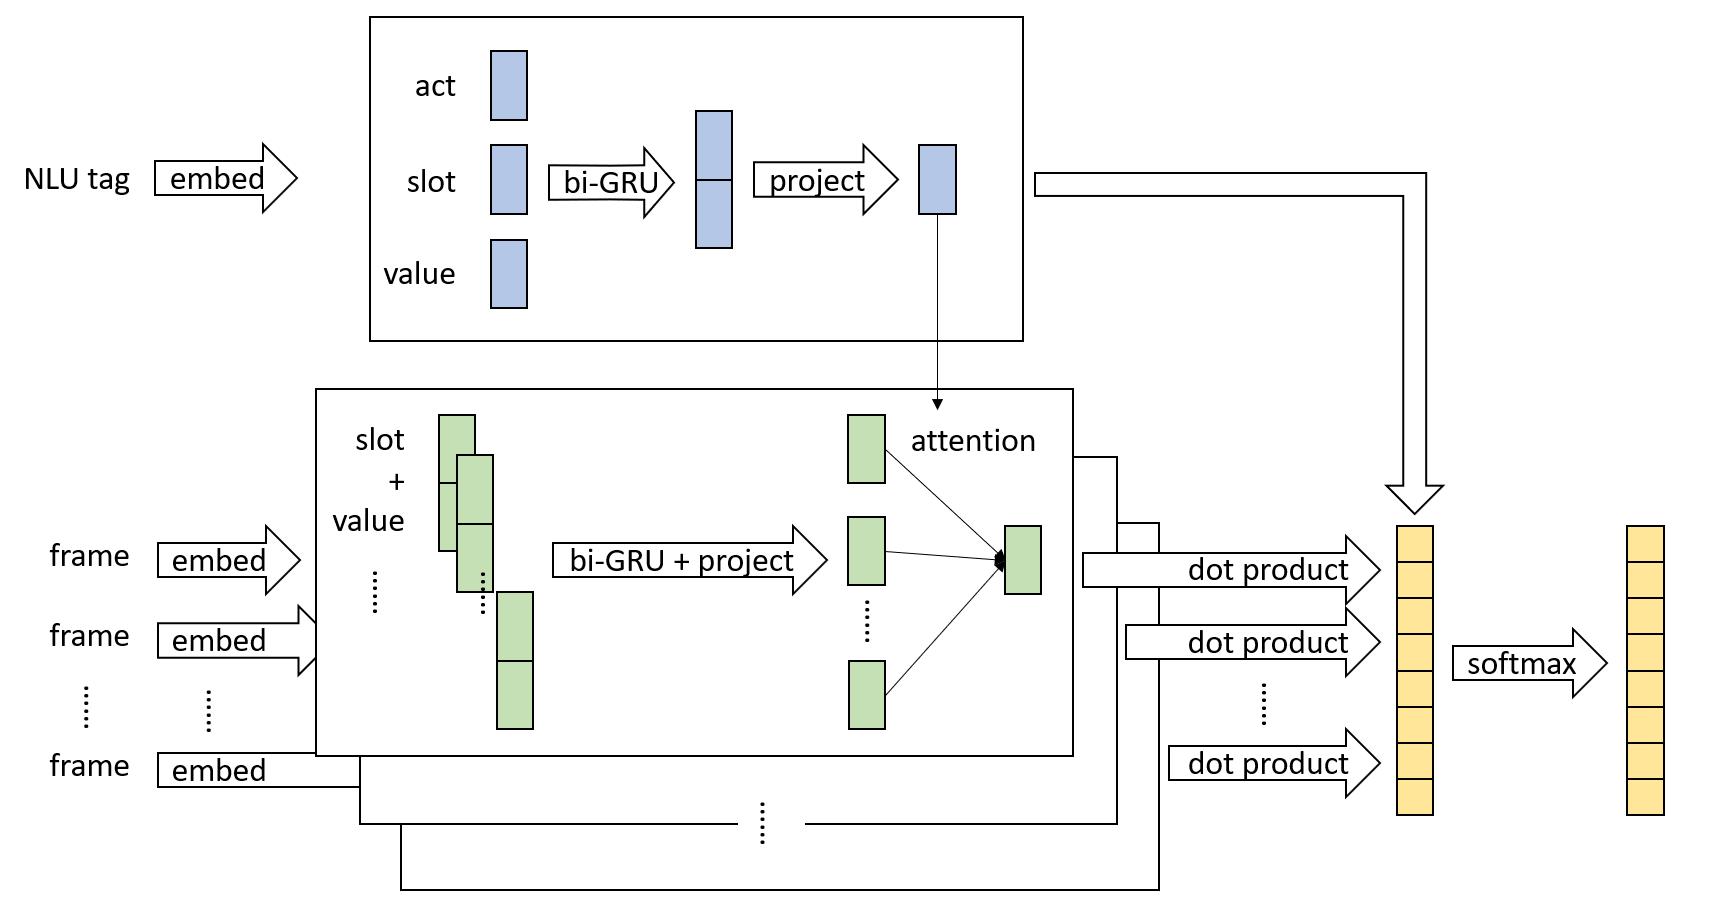
\includegraphics[width=\columnwidth]{model.png}
    \end{center}
}


%----------------------------------------------------------------------------------------
%	RESULTS
%----------------------------------------------------------------------------------------
\headerbox{Results}{name=results,column=1,below=model,span=1}{
    \begin{itemize}
        \item We evaluate the model by the accuracy of frame reference prediction on FRAMES dataset.
        \item The model achieves $83.1\%$ accuracy after hyperparameter tuning.
    \end{itemize}
    \begin{center}
            \begin{tabular}{lrr}
            \toprule
            Methods & No attention & Attention (dot product) \\
            \midrule
            Random & $58.1 \pm 0.22$ & - \\
            Maluuba \cite{schulz2017frame} & $76.4 \pm 4.49$ & -\\
            BERT w/o shuffle & $77.5 \pm 0.52$ & $81.0 \pm 0.69$ \\
            GRU w/o shuffle & $79.3 \pm 0.28$ & $81.9 \pm 1.05$ \\
            BERT w/ shuffle & $81.0 \pm 0.73$ & $82.3 \pm 1.70$ \\
            GRU w/ shuffle & $79.5 \pm 0.65$ & $\bm{82.8 \pm 0.52}$ \\
            \bottomrule
        \end{tabular}
    \end{center}
    \begin{center}
        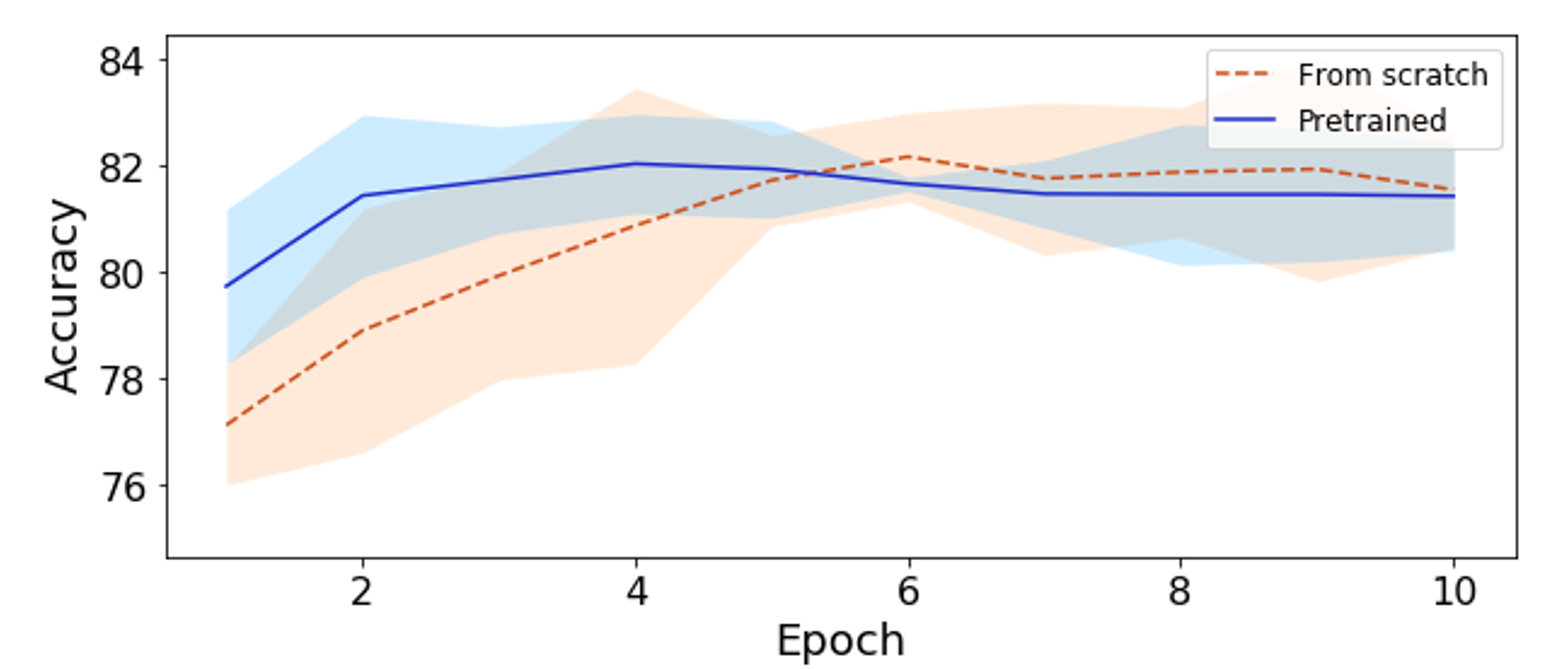
\includegraphics[width=\columnwidth]{curve.png}
    \end{center}
}


%----------------------------------------------------------------------------------------
%	CONCLUSION
%----------------------------------------------------------------------------------------
\headerbox{Conclusion}{name=conclusion,column=0,below=results,span=2}{
\begin{itemize}
    \item We propose a frame tracking model with attention mechanism, and improve the accuracy by $6.7$ percentage point.
    \item The model pre-trained on synthetic frame tracking data converges faster comparing to the model training from scratch.
\end{itemize}
}


%----------------------------------------------------------------------------------------
%	REFERENCES
%----------------------------------------------------------------------------------------
\headerbox{References}{name=reference,column=0,above=bottom,span=2}{
    \smaller  % Make the whole text smaller
    \bibliographystyle{plain}  % Use plain style
    \renewcommand{\section}[2]{\vskip 0.05em}  % Omit "References" title
    \bibliography{biblio}  % Use biblio.bib as the bibliography file
} 

\end{poster}
\end{document}